\documentclass[a4paper,11pt]{article}

\usepackage[english]{babel}
\usepackage[T1]{fontenc}
\usepackage{lmodern}
\usepackage{amsmath,amssymb}
\usepackage{graphicx}
\usepackage{booktabs}
\usepackage{array}
\usepackage{float}
\usepackage{microtype}
\usepackage{xcolor}
\usepackage{hyperref}
\usepackage[left=2cm,right=2cm,top=2cm,bottom=2cm]{geometry}

\graphicspath{{../figures/}}
\hypersetup{colorlinks=true,linkcolor=blue!50!black,urlcolor=blue!60!black,citecolor=blue!50!black}

\title{Comparative Optimization of the Rosenbrock Function}
\author{Florian Barbe}
\date{}

\begin{document}
\maketitle

\begin{abstract}
This report studies the generalized Rosenbrock objective through analytical
derivatives, a nonlinear least-squares formulation, and seven iterative
optimization configurations implemented directly in MATLAB. The experiments
use the two-dimensional case with $b=2$, Armijo backtracking with reduction
factor $0.75$, and the tolerances specified in the exercise. Numerical results
are reported without treating stagnation or divergence as convergence.
\end{abstract}

\section{Analytical properties}

For $x\in\mathbb{R}^n$ and $b>0$, the generalized Rosenbrock objective is
\begin{equation}
 f(x)=\sum_{i=1}^{n-1}\left[b(x_{i+1}-x_i^2)^2+(1-x_i)^2\right].
 \label{eq:objective}
\end{equation}
The first and last components of its gradient are
\begin{align}
 g_1&=-4bx_1(x_2-x_1^2)-2(1-x_1),\\
 g_n&=2b(x_n-x_{n-1}^2),
\end{align}
while, for $1<i<n$,
\begin{equation}
 g_i=2b(x_i-x_{i-1}^2)-4bx_i(x_{i+1}-x_i^2)-2(1-x_i).
\end{equation}

The Hessian is symmetric and tridiagonal. Its nonzero entries are
\begin{align}
 H_{1,1}&=2-4b(x_2-3x_1^2),\\
 H_{i,i}&=2+2b-4b(x_{i+1}-3x_i^2), &&1<i<n,\\
 H_{n,n}&=2b,\\
 H_{i,i+1}&=H_{i+1,i}=-4bx_i, &&1\leq i<n.
\end{align}

Every term in \eqref{eq:objective} is nonnegative. The value zero is reached
only if $1-x_i=0$ and $x_{i+1}-x_i^2=0$ for every $i<n$. Therefore the unique
global minimizer is
\begin{equation}
 x^\star=(1,\ldots,1)^T,\qquad f(x^\star)=0.
\end{equation}

\subsection{Nonlinear least-squares form}

Define $r(x)\in\mathbb{R}^{2n-2}$ by
\begin{equation}
 r_{2i-1}(x)=\sqrt{b}(x_{i+1}-x_i^2),\qquad
 r_{2i}(x)=1-x_i,qquad 1\leq i<n.
\end{equation}
Then $f(x)=r(x)^Tr(x)$. The Jacobian
$J(x)\in\mathbb{R}^{(2n-2)\times n}$ is rectangular and sparse. For each
$i=1,\ldots,n-1$, its only nonzero entries in rows $2i-1$ and $2i$ are
\begin{equation}
 J_{2i-1,i}=-2\sqrt{b}\,x_i,qquad
 J_{2i-1,i+1}=\sqrt{b},qquad
 J_{2i,i}=-1.
\end{equation}
With the convention $f=r^Tr$, the gradient identity is
\begin{equation}
 \nabla f(x)=2J(x)^Tr(x).
\end{equation}

Central finite differences were evaluated at two deterministic points for
$n=2,3,$ and $5$. The largest relative discrepancy among the gradient,
Hessian, Jacobian, and least-squares identity checks was below
$1.7\times10^{-10}$. This verification does not require the Symbolic Math
Toolbox.

\section{Objective visualization}

The experiments use $n=2$ and $b=2$. The objective was sampled with spacing
$0.05$ over $x_1\in[-4,4]$ and $x_2\in[-5,20]$.

\begin{figure}[H]
 \centering
 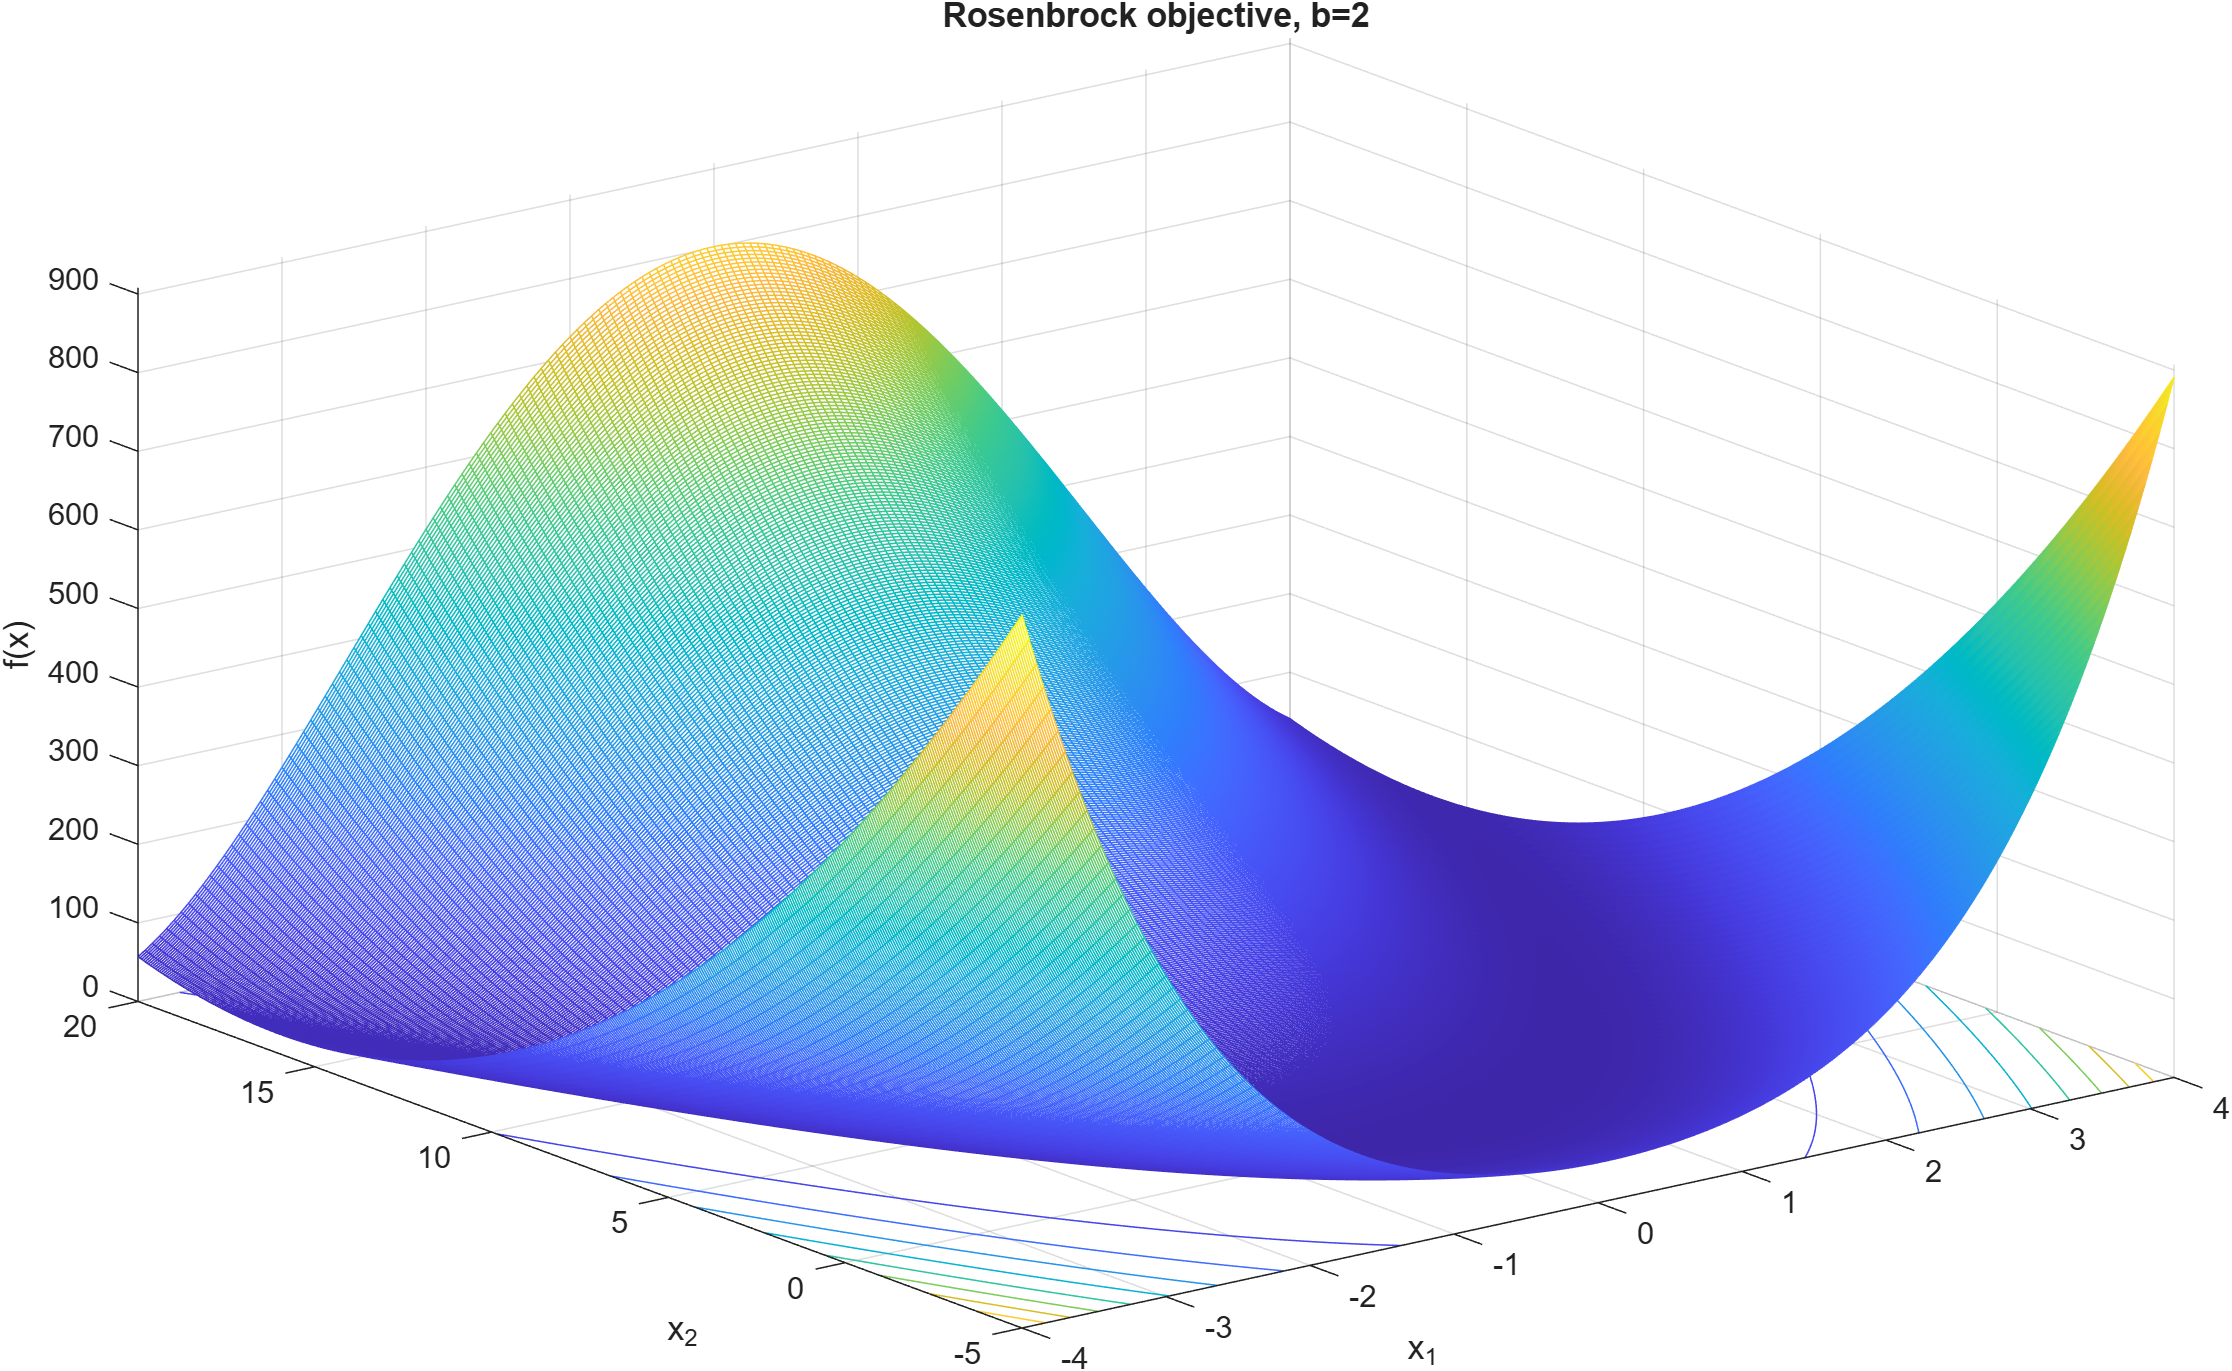
\includegraphics[width=0.78\textwidth]{partie1_01_rosenbrock_surface.png}
 \caption{Surface and projected contours of the Rosenbrock objective for $b=2$.}
 \label{fig:surface}
\end{figure}

\begin{figure}[H]
 \centering
 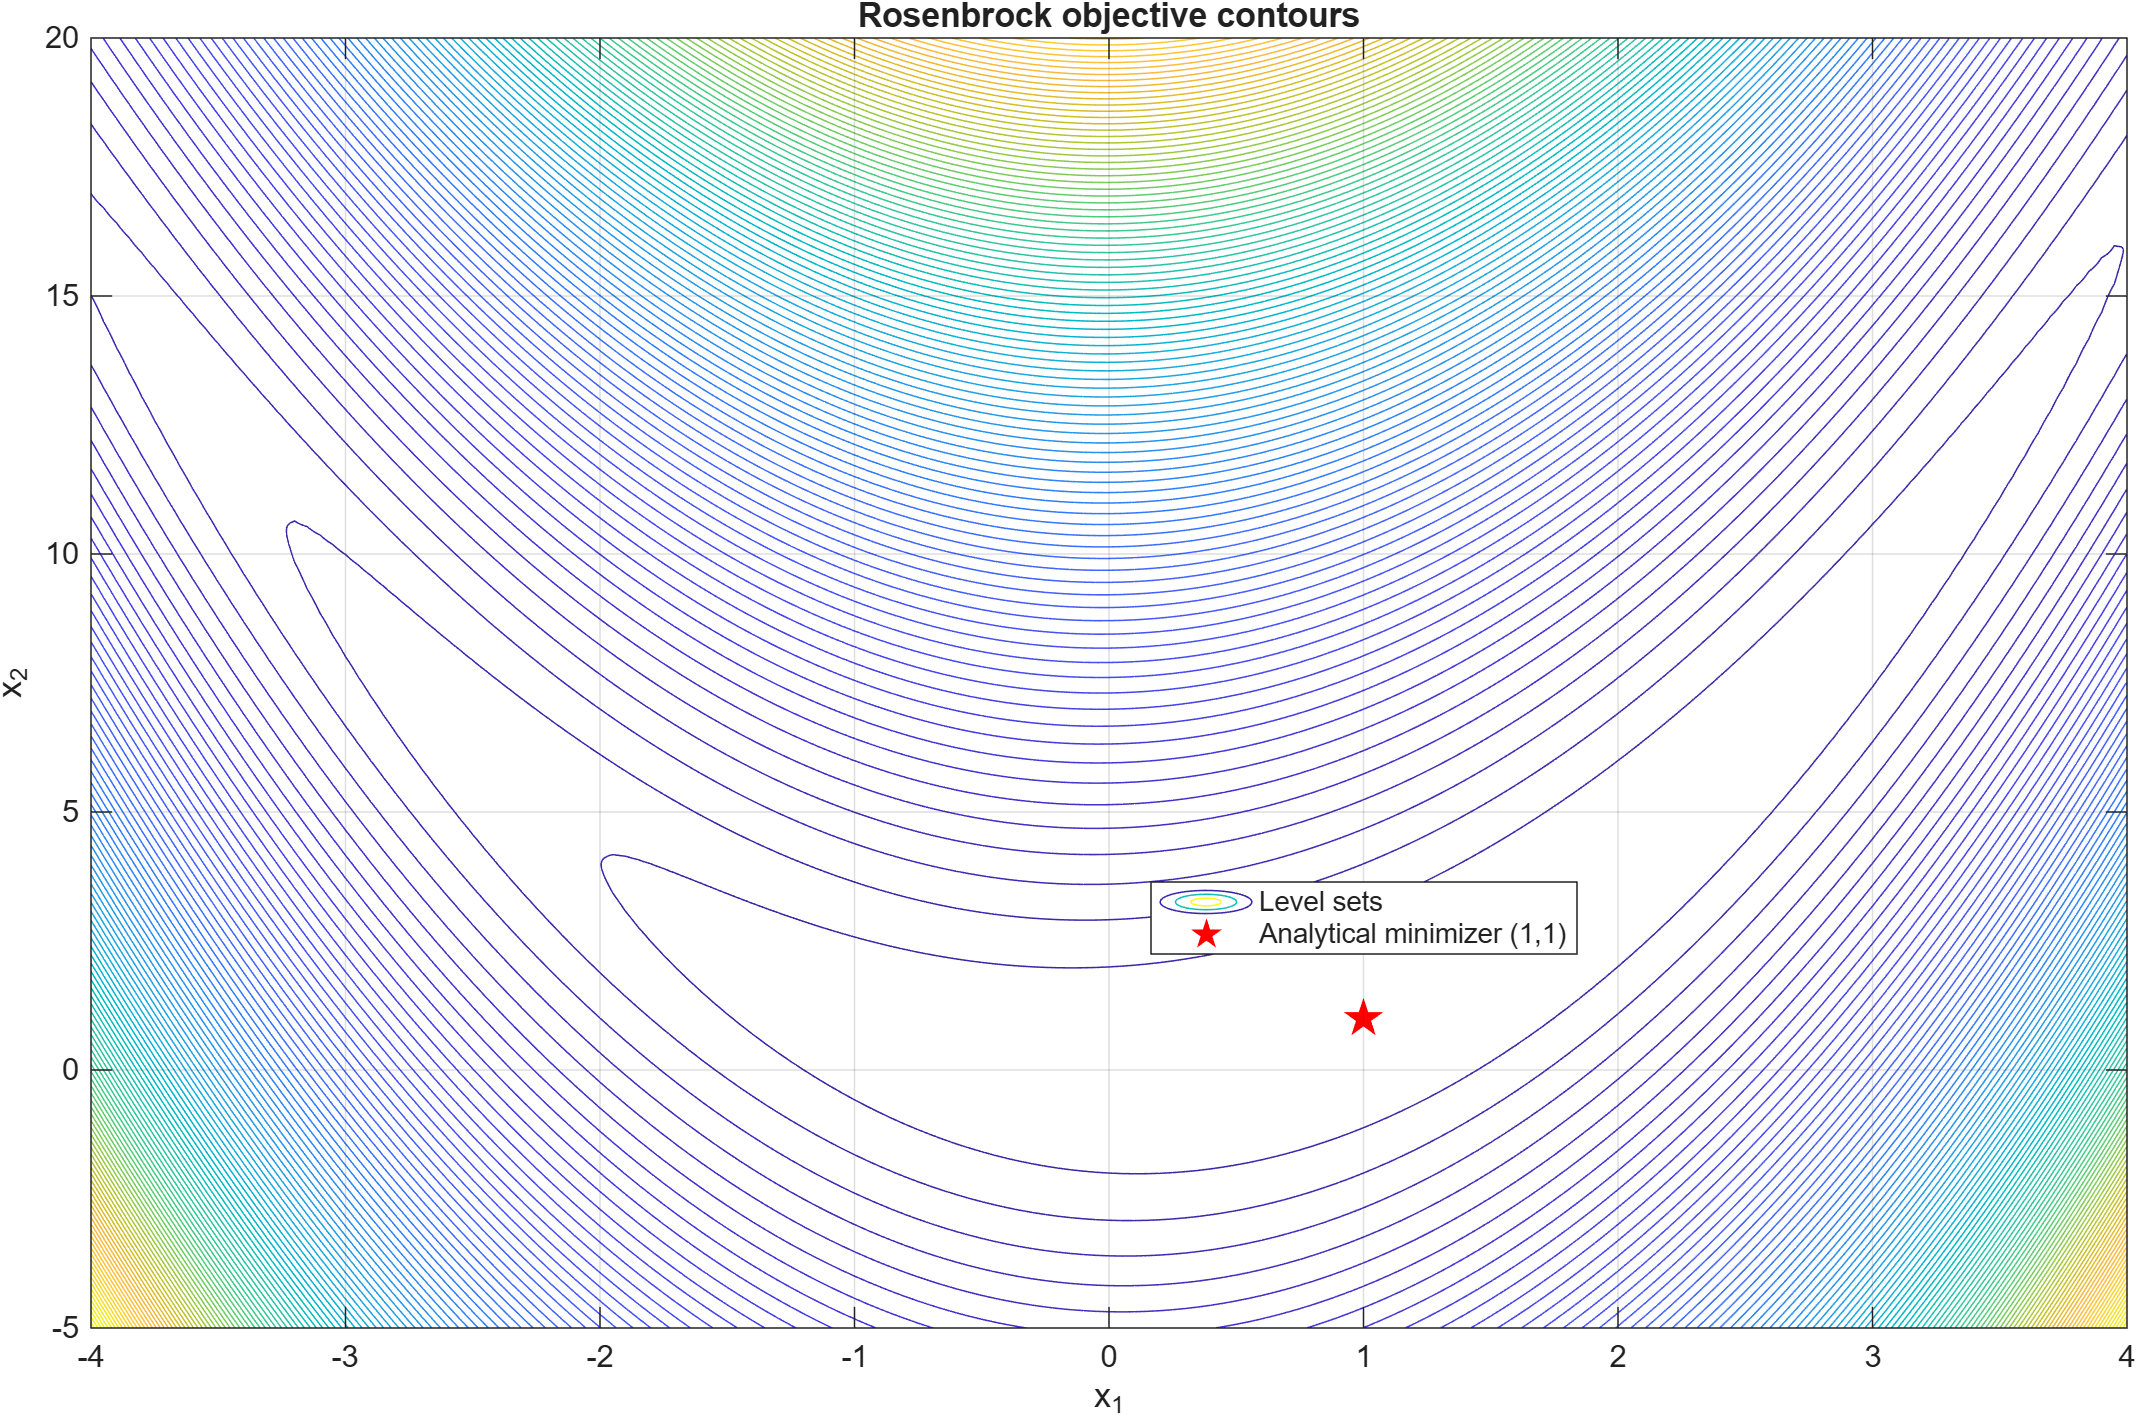
\includegraphics[width=0.72\textwidth]{partie1_02_rosenbrock_contours.png}
 \caption{One hundred level sets and the analytical minimizer $(1,1)^T$.}
 \label{fig:contours}
\end{figure}

Figures~\ref{fig:surface} and \ref{fig:contours} show the narrow curved valley
that makes the problem sensitive to both the direction and the step length.

\section{Fixed-step gradient descent}

Starting from $x_0=(0,0)^T$, three fixed steps were tested with at most
$1000$ iterations. Relative changes are defined by
\begin{equation}
 \delta_x=\frac{\lVert x_{k+1}-x_k\rVert_2}{\max(1,\lVert x_k\rVert_2)},
 \qquad
 \delta_f=\frac{|f_{k+1}-f_k|}{\max(1,|f_k|)}.
\end{equation}

\begin{table}[H]
\centering
\caption{Fixed-step gradient descent from $x_0=(0,0)^T$.}
\label{tab:fixed}
\begin{tabular}{rrrrrl}
\toprule
Step & $x_1$ & $x_2$ & $f(x)$ & $\lVert g\rVert_2$ & Stop \\
\midrule
$1$       & $-64.0000$ & $16.0000$ & $3.330\times10^7$ & $2.089\times10^6$ & Divergence \\
$10^{-2}$ & $0.9924$ & $0.9833$ & $6.257\times10^{-5}$ & $6.842\times10^{-3}$ & MaxIter \\
$10^{-4}$ & $0.1802$ & $0.0041$ & $6.737\times10^{-1}$ & $1.603$ & MaxIter \\
\bottomrule
\end{tabular}
\end{table}

\begin{figure}[H]
 \centering
 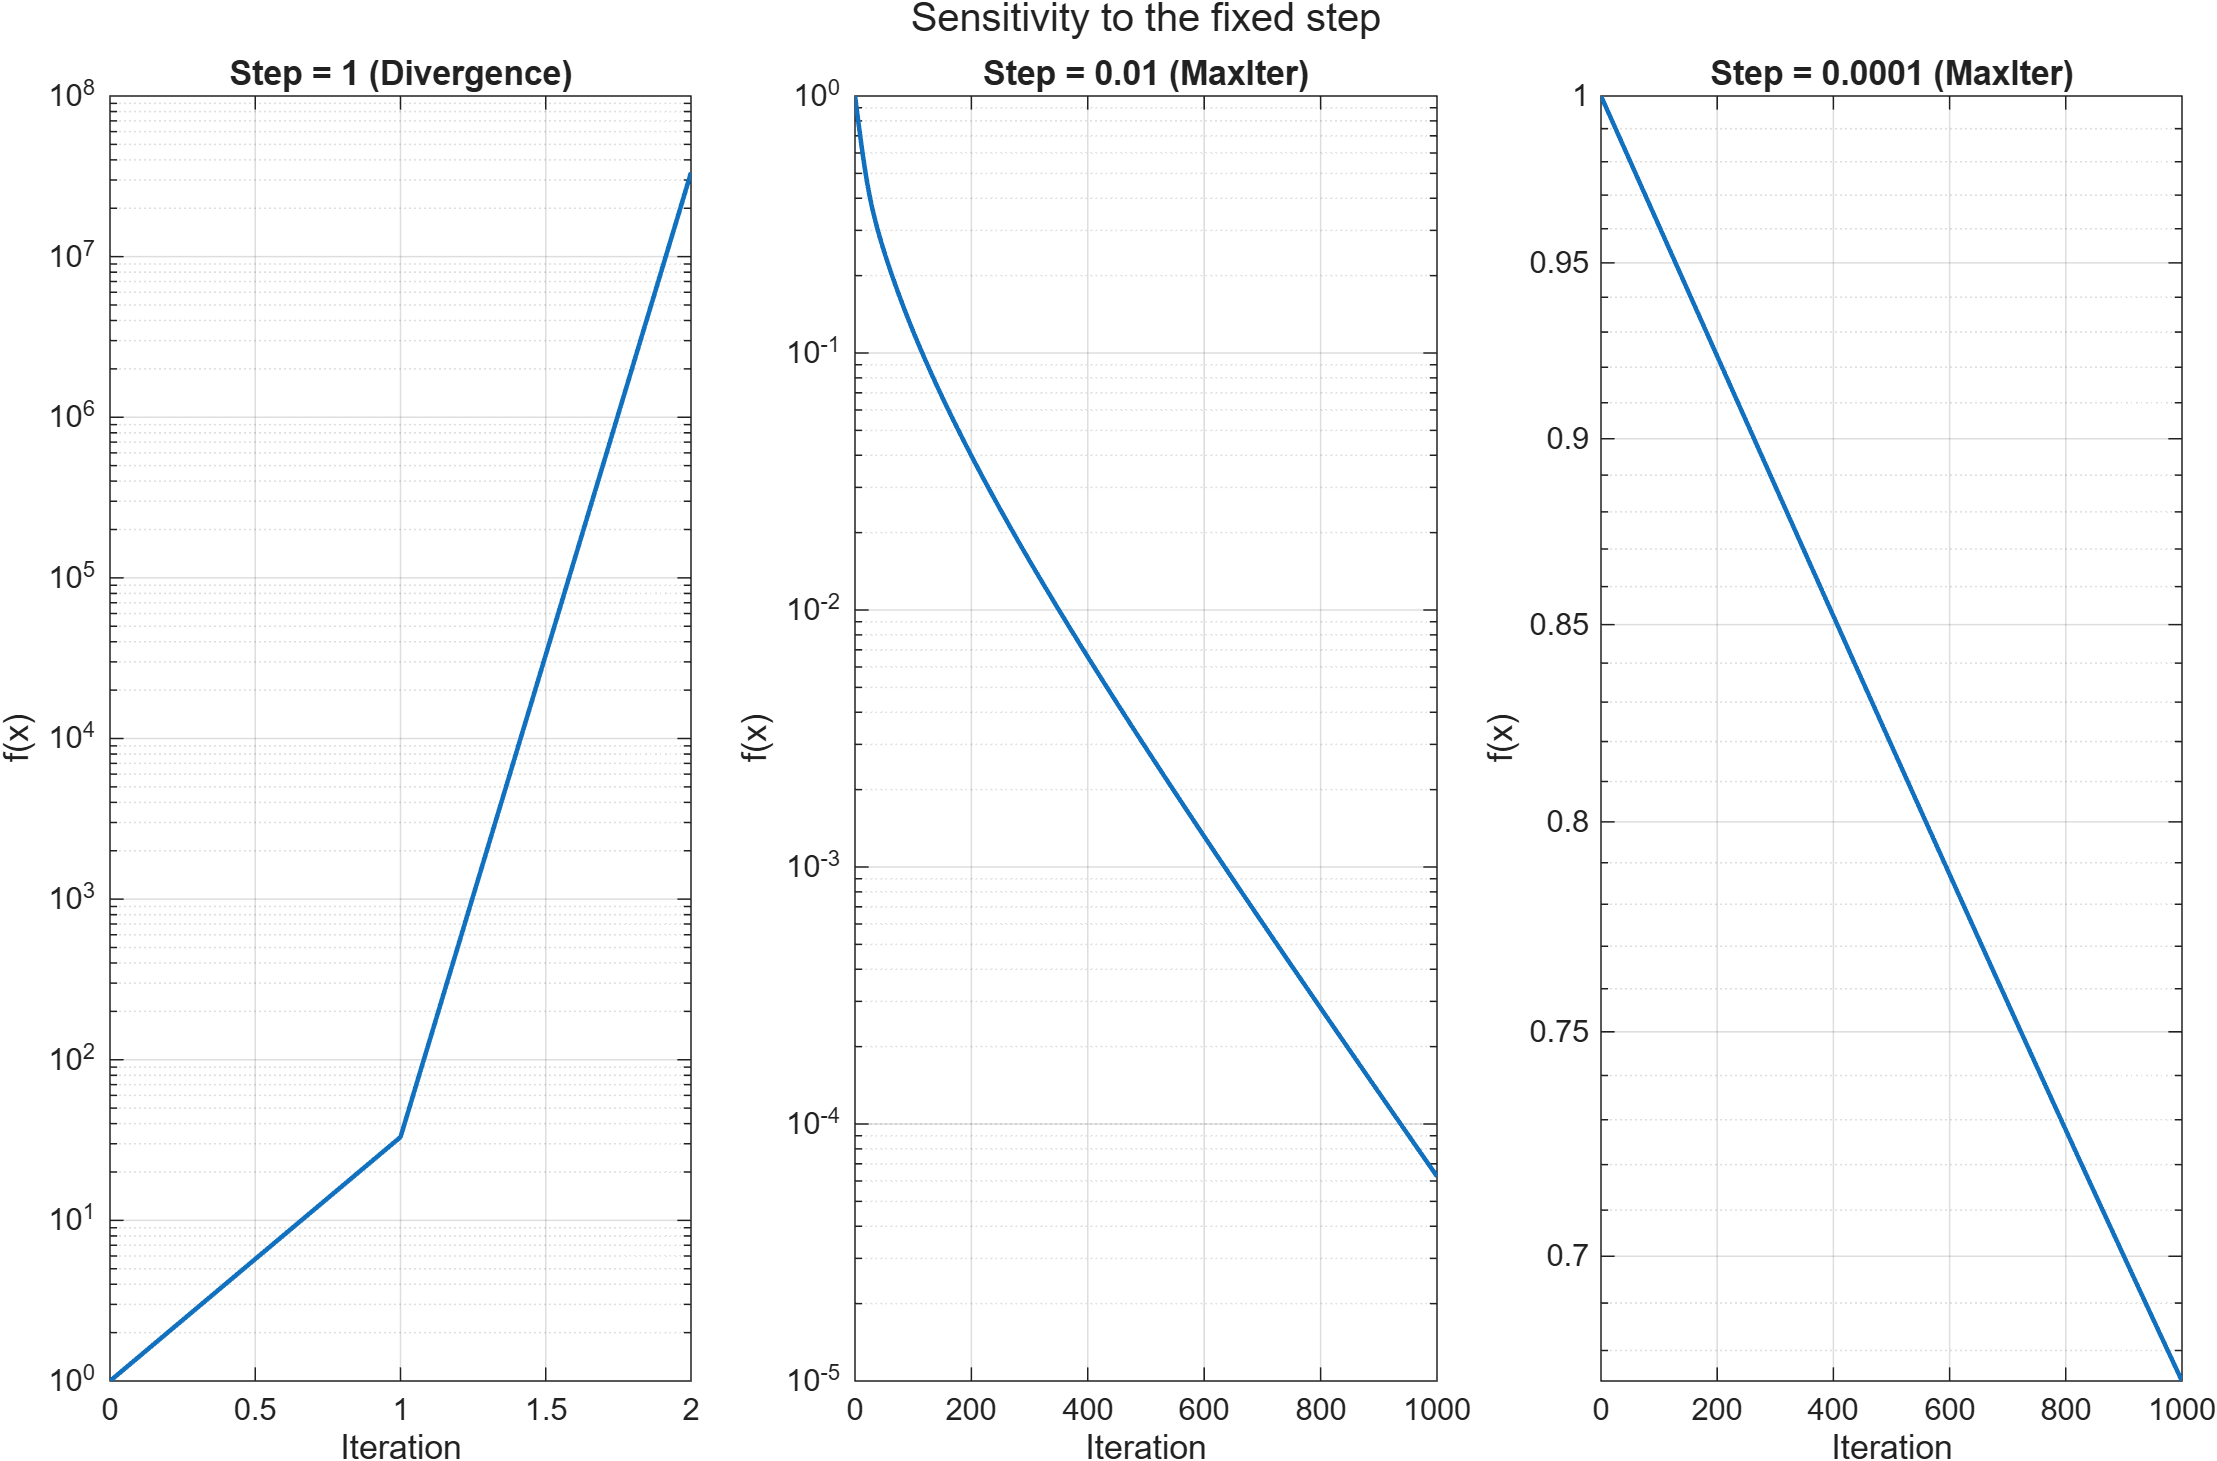
\includegraphics[width=\textwidth]{partie1_03_rosenbrock_pas_fixes.png}
 \caption{Objective histories for the three fixed steps. Divergence is retained rather than hidden.}
 \label{fig:fixed}
\end{figure}

The unit step is unstable from this starting point. The step $10^{-2}$ makes
substantial progress but does not satisfy a stopping tolerance within the
iteration limit. The smaller step $10^{-4}$ is stable but progresses too
slowly. Figure~\ref{fig:fixed} illustrates the sensitivity that motivates an
adaptive line search.

\section{Armijo backtracking}

For a descent direction $d_k$, the accepted step satisfies
\begin{equation}
 f(x_k+\alpha_kd_k)\leq f(x_k)+c\alpha_k g_k^Td_k,
 \qquad c=10^{-4}.
\end{equation}
The search starts from $\alpha=1$ and multiplies it by $0.75$ after a failed
trial. Stopping tests are applied only after a trial has been accepted.

From $(0,0)^T$, gradient descent with Armijo reaches
$x=(0.998729,0.996562)^T$ after $139$ iterations, with
$f=3.226\times10^{-6}$ and $\lVert g\rVert_2=5.858\times10^{-3}$. The stop is
\texttt{TolF}, not \texttt{TolG}; it must therefore be interpreted as
stagnation in the objective rather than full first-order convergence.

\begin{figure}[H]
 \centering
 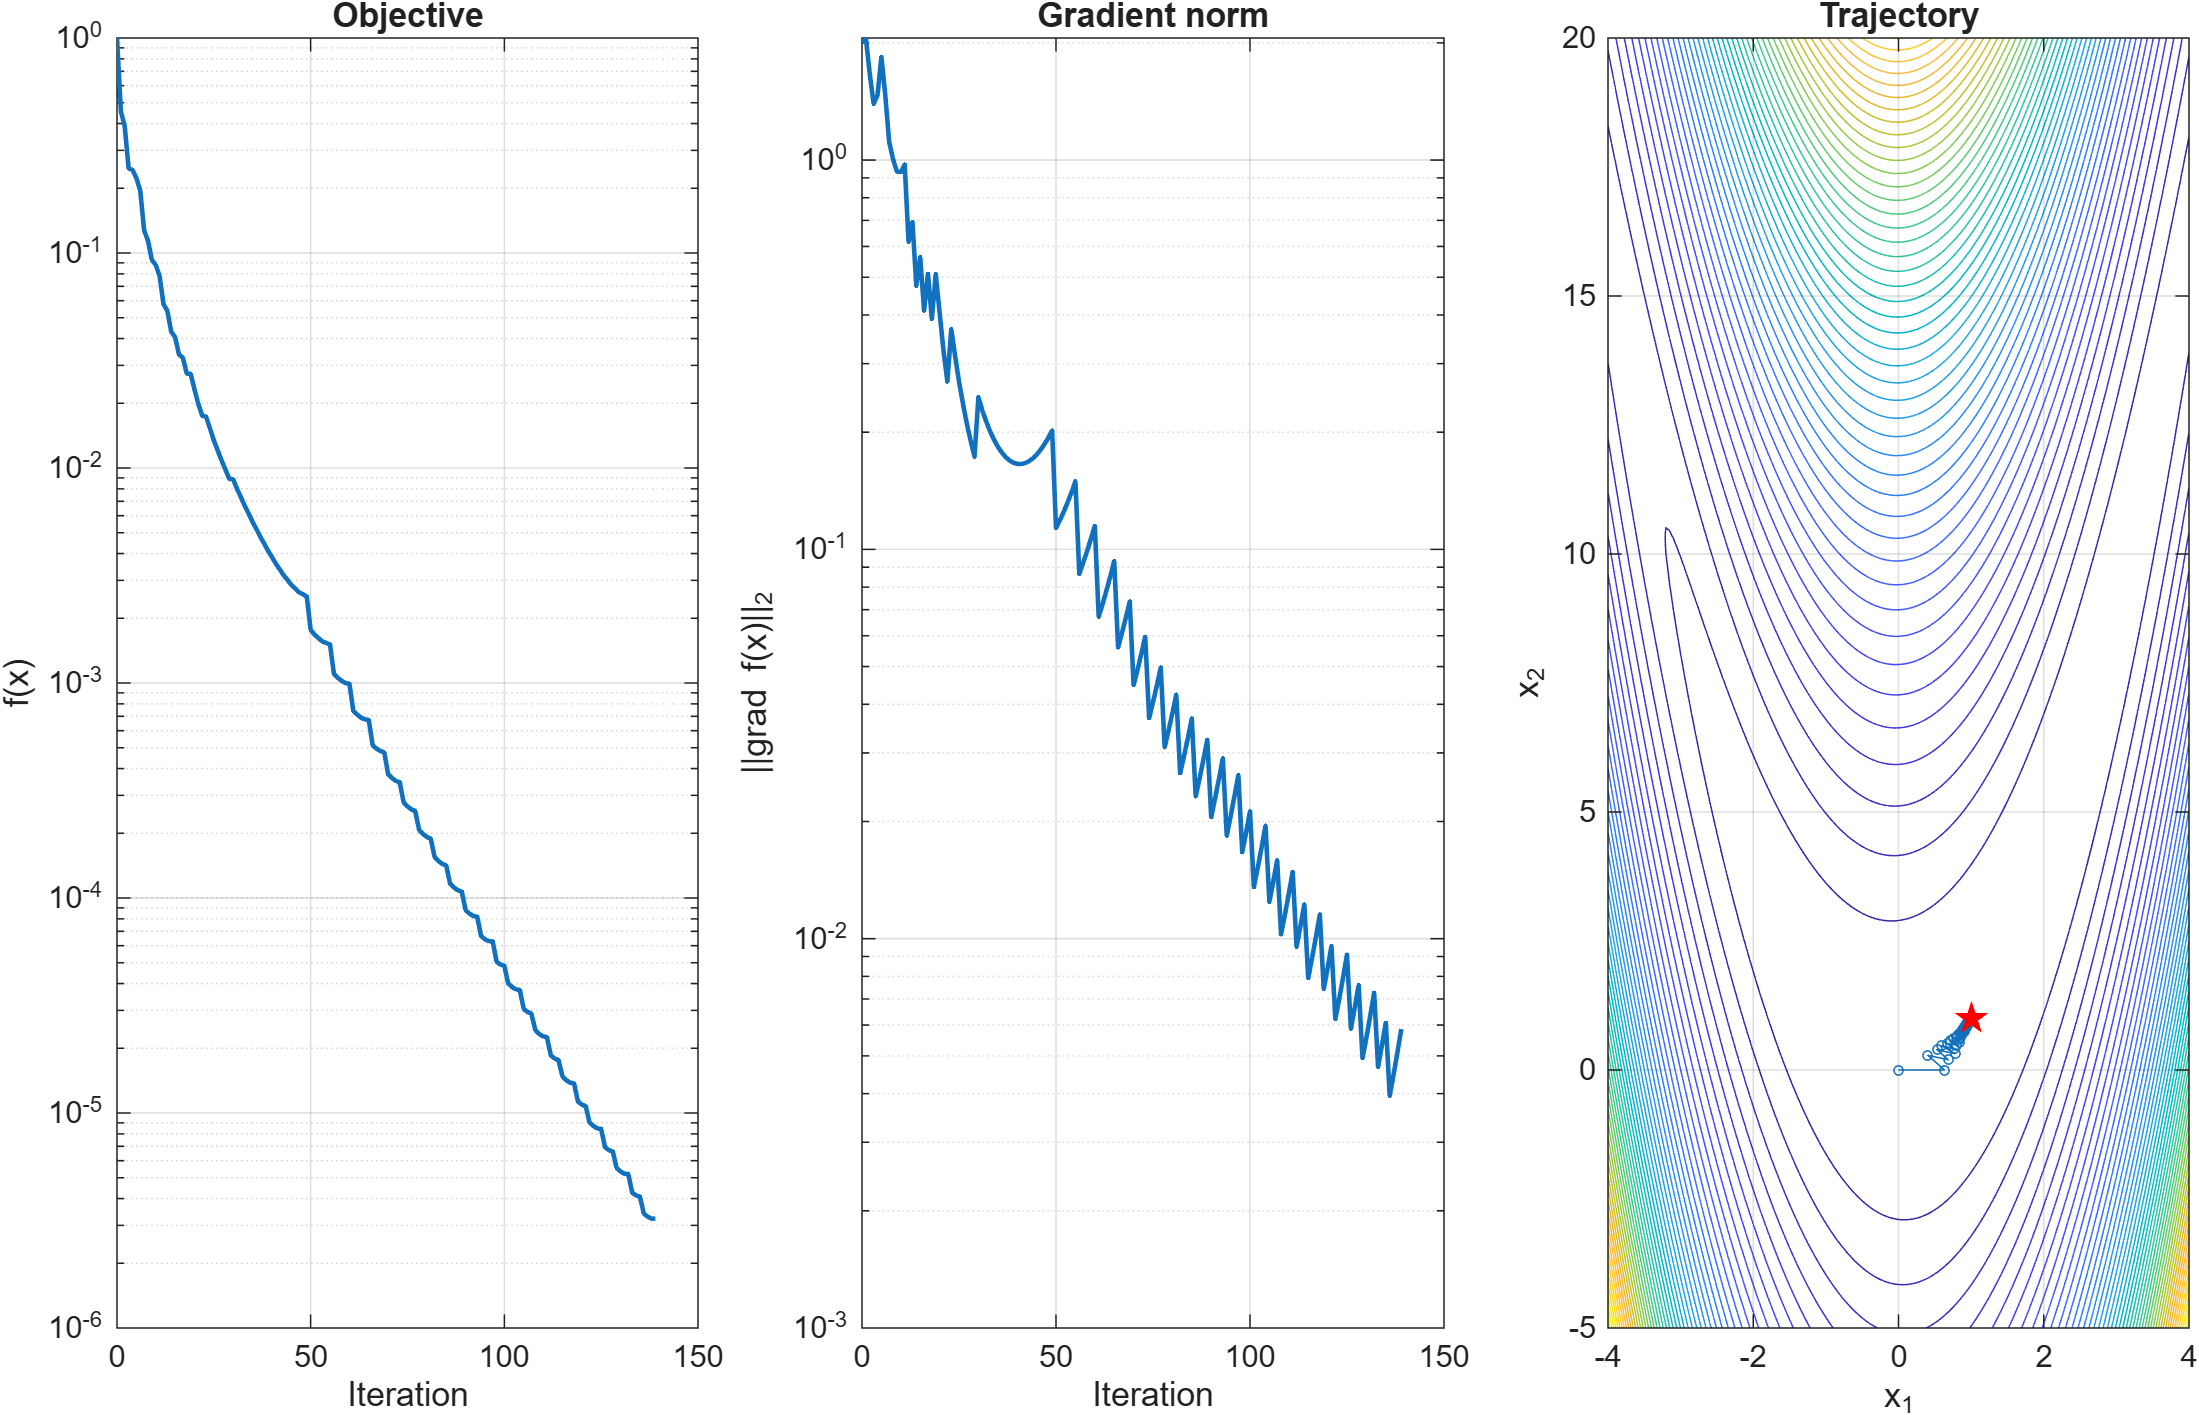
\includegraphics[width=\textwidth]{partie1_05_rosenbrock_armijo.png}
 \caption{Objective, gradient norm, and trajectory for gradient descent with Armijo backtracking.}
 \label{fig:armijo}
\end{figure}

\section{Comparison of optimization methods}

The seven configurations are gradient descent with Armijo, nonlinear
Fletcher--Reeves, Newton with a unit step, Newton with Armijo, inverse-BFGS,
Gauss--Newton, and Levenberg--Marquardt. Every run reinitializes its internal
state from the same starting vector. When the Newton Hessian is not positive
definite, a diagonal spectral shift is added before solving the Newton system.
BFGS is restarted with the identity matrix if its curvature condition fails.

Gauss--Newton solves a regularized version of
$(J^TJ)d=-J^Tr$. Levenberg--Marquardt solves
$(J^TJ+\mu I)d=-J^Tr$ and accepts a trial using the ratio between actual and
predicted reduction. The damping parameter decreases when this ratio is at
least $0.75$ and increases when it is at most $0.25$.

\begin{table}[H]
\centering
\caption{Results from $x_0=(-2,10)^T$. Times are single-run measurements and are only indicative.}
\label{tab:start1}
\resizebox{\textwidth}{!}{%
\begin{tabular}{lrrrrl}
\toprule
Method & $f(x)$ & $\lVert g\rVert_2$ & Iter. & Time (s) & Stop \\
\midrule
Gradient Armijo & $1.257\times10^{-5}$ & $1.128\times10^{-2}$ & 903 & 0.1314 & TolF \\
Fletcher--Reeves & $1.593\times10^{-7}$ & $1.226\times10^{-3}$ & 57 & 0.0917 & TolF \\
Newton unit step & $8.100\times10^{1}$ & $9.315\times10^{1}$ & 0 & 0.0987 & Divergence \\
Newton Armijo & $9.217\times10^{-29}$ & $5.939\times10^{-14}$ & 13 & 0.0138 & TolG \\
BFGS & $4.227\times10^{-17}$ & $5.618\times10^{-9}$ & 18 & 0.0195 & TolG \\
Gauss--Newton & $1.666\times10^{-22}$ & $1.217\times10^{-11}$ & 3 & 0.0050 & TolG \\
Levenberg--Marquardt & $8.089\times10^{-14}$ & $2.524\times10^{-7}$ & 5 & 0.0168 & TolF \\
\bottomrule
\end{tabular}}
\end{table}

\begin{table}[H]
\centering
\caption{Results from $x_0=(4,-5)^T$. Times are single-run measurements and are only indicative.}
\label{tab:start2}
\resizebox{\textwidth}{!}{%
\begin{tabular}{lrrrrl}
\toprule
Method & $f(x)$ & $\lVert g\rVert_2$ & Iter. & Time (s) & Stop \\
\midrule
Gradient Armijo & $2.181\times10^{-6}$ & $4.797\times10^{-3}$ & 149 & 0.0039 & TolF \\
Fletcher--Reeves & $2.601\times10^{-8}$ & $4.437\times10^{-4}$ & 74 & 0.0095 & TolF \\
Newton unit step & $6.174\times10^{-23}$ & $1.571\times10^{-11}$ & 5 & 0.0054 & TolG \\
Newton Armijo & $2.465\times10^{-32}$ & $9.930\times10^{-16}$ & 10 & 0.0012 & TolG \\
BFGS & $7.384\times10^{-14}$ & $1.343\times10^{-6}$ & 22 & 0.0054 & TolF \\
Gauss--Newton & $4.265\times10^{-20}$ & $1.947\times10^{-10}$ & 2 & 0.0059 & TolG \\
Levenberg--Marquardt & $1.313\times10^{-17}$ & $3.346\times10^{-9}$ & 4 & 0.0068 & TolG \\
\bottomrule
\end{tabular}}
\end{table}

\begin{figure}[H]
 \centering
 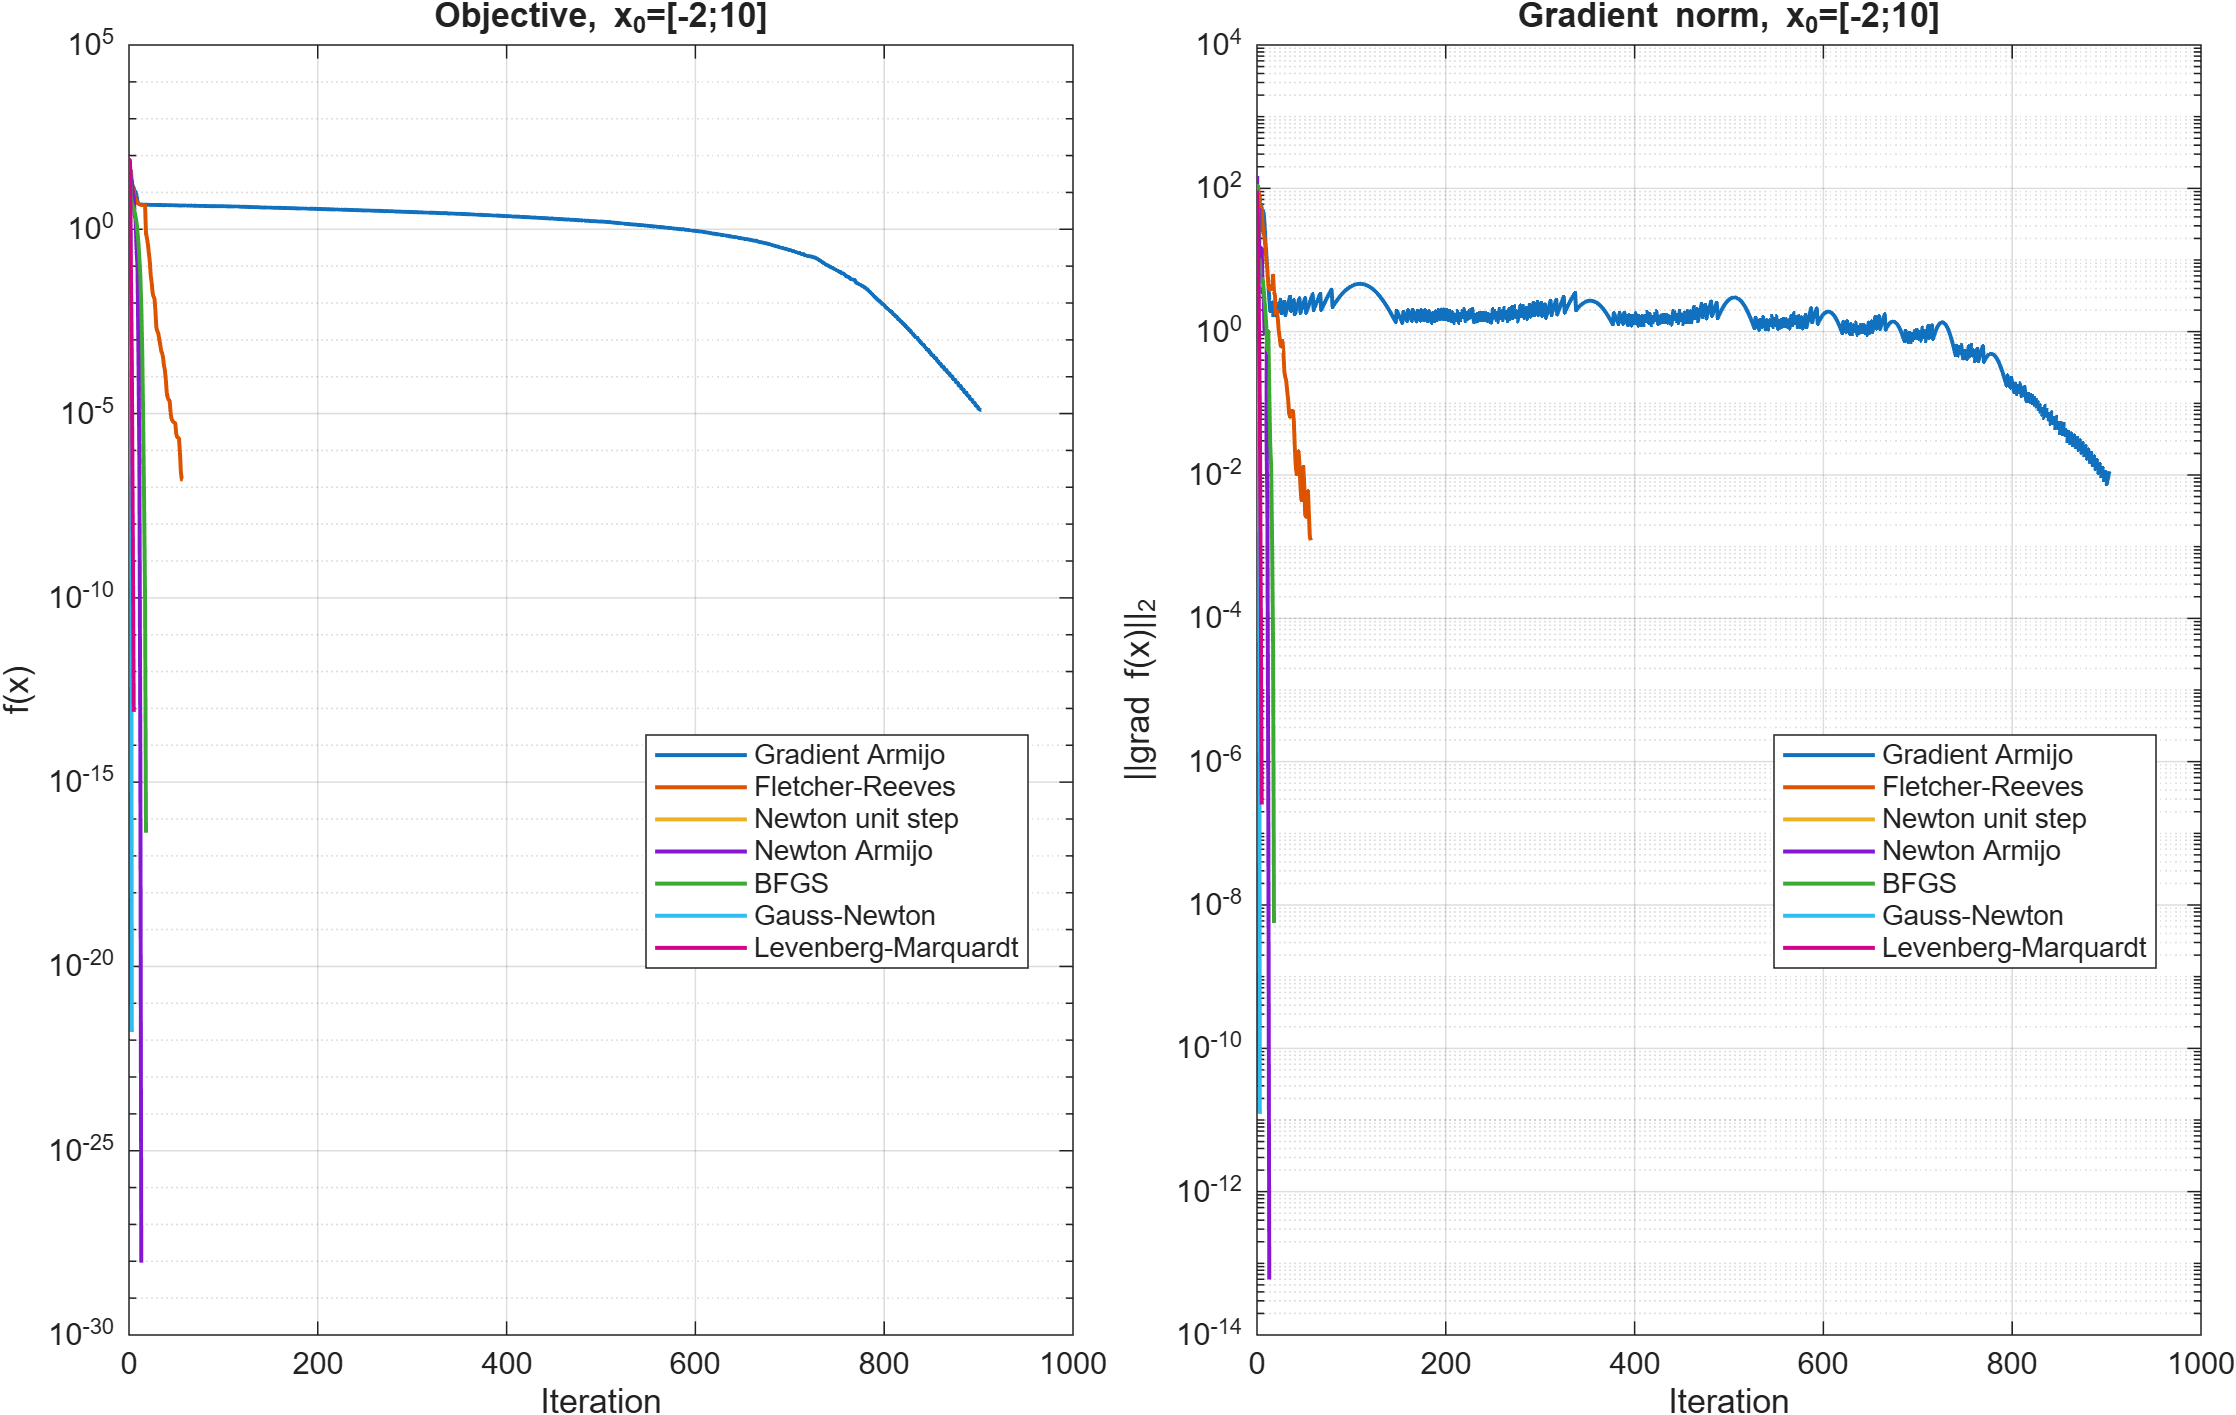
\includegraphics[width=\textwidth]{partie1_06_comparaison_rosenbrock_point_1.png}
 \caption{Objective and gradient histories from $x_0=(-2,10)^T$.}
 \label{fig:start1}
\end{figure}

\begin{figure}[H]
 \centering
 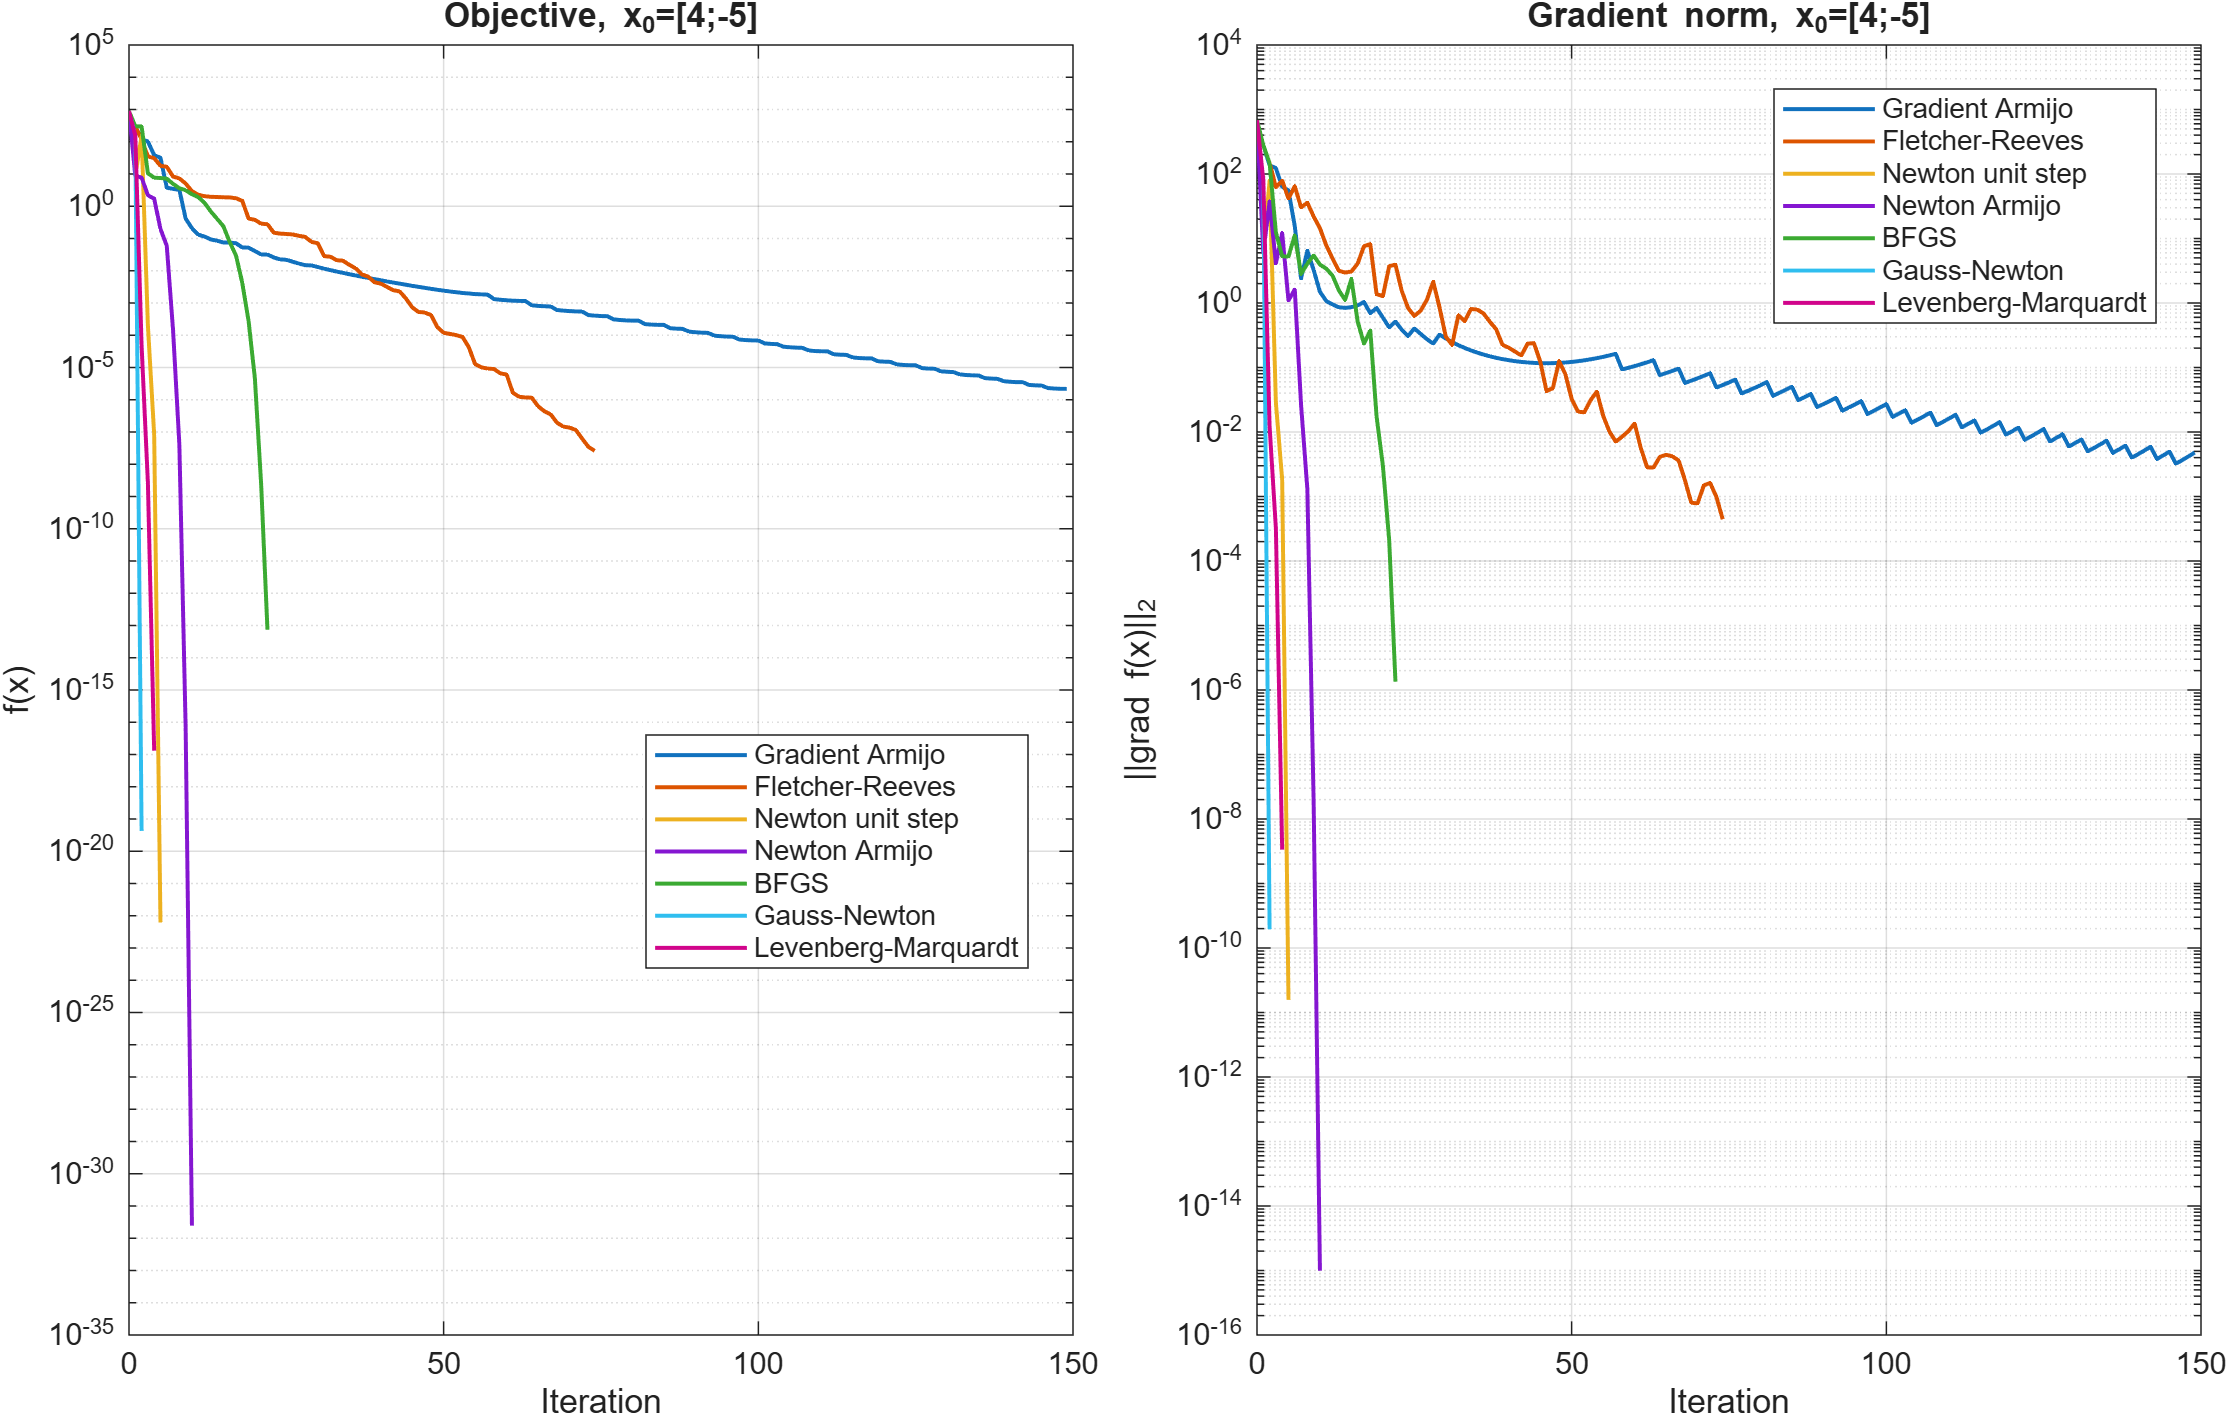
\includegraphics[width=\textwidth]{partie1_07_comparaison_rosenbrock_point_2.png}
 \caption{Objective and gradient histories from $x_0=(4,-5)^T$.}
 \label{fig:start2}
\end{figure}

The comparison in Figures~\ref{fig:start1} and \ref{fig:start2} exposes a
strong dependence on the starting point. The unit-step Newton method diverges
immediately from $(-2,10)^T$ but converges in five iterations from $(4,-5)^T$.
Armijo globalization removes this failure in the first case. The nonlinear
least-squares structure is especially favorable here: Gauss--Newton reaches
the gradient tolerance in two or three accepted iterations, while the damped
Levenberg--Marquardt method requires four or five. Gradient and
Fletcher--Reeves runs that stop on \texttt{TolF} still have visibly larger
gradient norms and should be described as stagnated rather than fully
converged.

\section{Conclusion}

The Rosenbrock valley illustrates why a fixed step cannot simultaneously
provide stability and fast progress over the full trajectory. Armijo
backtracking improves robustness, but first-order methods still require many
iterations. Curvature information substantially reduces the iteration count,
provided that indefinite Hessians and failed trial steps are handled. For this
specific objective, the residual representation gives Gauss--Newton and
Levenberg--Marquardt a decisive advantage. These conclusions concern only the
two-dimensional case with $b=2$ and the two prescribed starting points; they
are not a general ranking of optimization algorithms.

\begin{thebibliography}{9}

\bibitem{rosenbrock1960}
H. H. Rosenbrock,
``An automatic method for finding the greatest or least value of a function,''
\emph{The Computer Journal}, vol. 3, no. 3, pp. 175--184, 1960.
\url{https://doi.org/10.1093/comjnl/3.3.175}

\bibitem{armijo1966}
L. Armijo,
``Minimization of functions having Lipschitz continuous first partial derivatives,''
\emph{Pacific Journal of Mathematics}, vol. 16, no. 1, pp. 1--3, 1966.
\url{https://doi.org/10.2140/pjm.1966.16.1}

\bibitem{fletcherreeves1964}
R. Fletcher and C. M. Reeves,
``Function minimization by conjugate gradients,''
\emph{The Computer Journal}, vol. 7, no. 2, pp. 149--154, 1964.
\url{https://doi.org/10.1093/comjnl/7.2.149}

\bibitem{broyden1970}
C. G. Broyden,
``The convergence of a class of double-rank minimization algorithms: 1. General considerations,''
\emph{IMA Journal of Applied Mathematics}, vol. 6, no. 1, pp. 76--90, 1970.
\url{https://doi.org/10.1093/imamat/6.1.76}

\bibitem{levenberg1944}
K. Levenberg,
``A method for the solution of certain non-linear problems in least squares,''
\emph{Quarterly of Applied Mathematics}, vol. 2, no. 2, pp. 164--168, 1944.
\url{https://doi.org/10.1090/qam/10666}

\bibitem{marquardt1963}
D. W. Marquardt,
``An algorithm for least-squares estimation of nonlinear parameters,''
\emph{Journal of the Society for Industrial and Applied Mathematics}, vol. 11,
no. 2, pp. 431--441, 1963.
\url{https://doi.org/10.1137/0111030}

\end{thebibliography}

\end{document}
